\documentclass[12pt,letterpaper]{article}

\usepackage[margin=0.75in]{geometry}
\usepackage{amsmath,amssymb}
\usepackage{enumitem}
\usepackage{tikz}

\pagestyle{empty}
\setlength{\parindent}{0pt}
\setlength{\parskip}{0.5em}
\setlength{\emergencystretch}{2em}

\begin{document}

\begin{center}
  {\large\bfseries MATH 15200: Calculus II}\\
  {\large\bfseries Homework 3: Area and Volumes of Revolution}
\end{center}

\vspace{0.25em}
\hrule
\vspace{0.8em}

\textbf{Due:} Monday, October 19, 2026, at 11:59 PM.

This is the written portion of Homework 3; complete the routine online portion
separately in Edfinity. Upload your written solutions to Gradescope, via Canvas. You may
collaborate, but you must write and submit your own solutions independently.



\vspace{0.8em}


\begin{enumerate}[label=\textbf{\arabic*.},leftmargin=2em,itemsep=1.25em]
  \item Find the total area enclosed by the curves $y=x\sqrt{4-x^2}$ and
    $y=x$. Then evaluate
    \[
      \int_{-\sqrt{3}}^{\sqrt{3}}\bigl(x\sqrt{4-x^2}-x\bigr)\,dx,
    \]
    and explain why it is not equal to the area you found.

    \emph{Hint:} Find all points where the curves intersect, being careful
    not to lose a solution by dividing by $x$. Sketch both curves and, on
    each interval between consecutive intersection points, decide which curve
    lies above the other. To integrate $x\sqrt{4-x^2}$, use the substitution
    $u=4-x^2$.

  \item Find the volume of the solid formed by revolving the disk
    $x^2+y^2\le 1$ about the line $y=3$.

    \emph{Hint:} Use the ``washer method'' to revolve the upper and lower 
    semicircles. Set up the integral and simplify as far as you can. Then 
    notice that \(\int_{-1}^1 \sqrt{1-x^2} dx\) is the area of a 
    semicirle of radius 1. What is it equal to?

  \item A cylindrical hole is drilled straight through the center of a solid
    ball of radius $R$. The solid that remains is called a \emph{napkin ring}.
    Let $h$ be its height, i.e. the distance between the two circular openings. 
    Show that the volume of the napkin ring does not depend on $R$.

    \begin{center}
      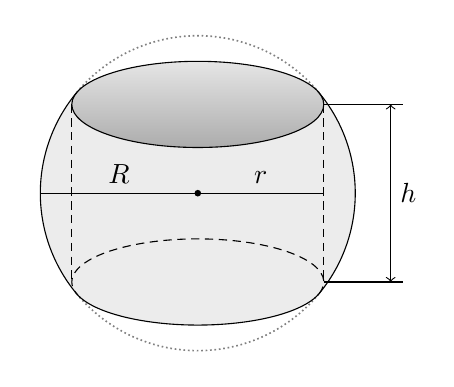
\begin{tikzpicture}[
          hidden/.style={densely dashed, thin},
          ghost/.style={gray, densely dotted, semithick},
        ]
        % Ball radius, h/2, and viewing elevation in degrees; the rest is
        % derived from these.
        \pgfmathsetmacro{\ballR}{2}
        \pgfmathsetmacro{\halfH}{1.2}
        \pgfmathsetmacro{\elev}{20}
        \pgfmathsetmacro{\holeR}{sqrt(\ballR^2-\halfH^2)}
        \pgfmathsetmacro{\rimC}{\halfH*cos(\elev)}
        \pgfmathsetmacro{\rimB}{\holeR*sin(\elev)}
        \pgfmathsetmacro{\outA}{asin(\halfH/(\ballR*cos(\elev)))}
        \pgfmathsetmacro{\rimA}{asin(\halfH*tan(\elev)/\holeR)}
        % Outer surface, and the inside of the hole seen through the top.
        \fill[gray!15]
          (-\outA:\ballR) arc[start angle=-\outA, end angle=\outA,
                              radius=\ballR]
          arc[start angle=\rimA, end angle=180-\rimA,
              x radius=\holeR, y radius=\rimB]
          arc[start angle=180-\outA, end angle=180+\outA, radius=\ballR]
          arc[start angle=180+\rimA, end angle=360-\rimA,
              x radius=\holeR, y radius=\rimB]
          -- cycle;
        \shade[top color=gray!20, bottom color=gray!65]
          (0,\rimC) ellipse[x radius=\holeR, y radius=\rimB];
        % Caps removed from the ball.
        \draw[ghost] (\outA:\ballR)
          arc[start angle=\outA, end angle=180-\outA, radius=\ballR];
        \draw[ghost] (180+\outA:\ballR)
          arc[start angle=180+\outA, end angle=360-\outA, radius=\ballR];
        % Hidden edges.
        \draw[hidden] (-\outA:\ballR)
          arc[start angle=-\rimA, end angle=180+\rimA,
              x radius=\holeR, y radius=\rimB];
        \draw[hidden] (\holeR,\rimC) -- (\holeR,-\rimC);
        \draw[hidden] (-\holeR,\rimC) -- (-\holeR,-\rimC);
        % Visible edges.
        \draw (0,\rimC) ellipse[x radius=\holeR, y radius=\rimB];
        \draw (-\outA:\ballR)
          arc[start angle=-\outA, end angle=\outA, radius=\ballR];
        \draw (180-\outA:\ballR)
          arc[start angle=180-\outA, end angle=180+\outA, radius=\ballR];
        \draw (180+\outA:\ballR)
          arc[start angle=180+\rimA, end angle=360-\rimA,
              x radius=\holeR, y radius=\rimB];
        % Labels.
        \fill (0,0) circle[radius=1.2pt];
        \draw (0,0) -- node[above] {$R$} (180:\ballR);
        \draw (0,0) -- node[above] {$r$} (\holeR,0);
        \draw[thin] (\holeR,\rimC) -- (\ballR+0.6,\rimC);
        \draw[thin] (\holeR,-\rimC) -- (\ballR+0.6,-\rimC);
        \draw[<->] (\ballR+0.45,-\rimC) -- node[right] {$h$}
          (\ballR+0.45,\rimC);
      \end{tikzpicture}
    \end{center}

    \emph{Hint:} Place the center of the ball at the origin, with the hole
    along the $y$-axis, and let $r$ be the radius of the hole. Then the napkin
    ring is the solid formed by revolving the region of points $(x,y)$ with
    $x^2+y^2\le R^2$ and $x\ge r$ about the $y$-axis. Explain why
    $R^2-r^2=h^2/4$. Then find the outer and inner radii of the rotated cross-section 
    at height $y$, for $-h/2\le y\le h/2$.


\end{enumerate}

\end{document}
